\chapter{Code structure}

%====================================================================
% Directory structure.
%====================================================================

\section{Directory structure}

Figure \ref{F:directory_structure} illustrates the directory structure of \SES. The contents of the different directories are as
follows:\\[5pt]
\texttt{ADJOINT:} Adjoint source time functions and a list of adjoint source locations.\\[5pt]
\texttt{DATA/COORDINATES:} ASCII files containing the grid point coordinates for each model subdomain.\\[5pt]
\texttt{DATA/LOGFILES:} Logfiles for each model subdomain. Logfiles document the geometrical setup of each subdomain and the iteration progress. They are mostly used for debugging.\\[5pt]
\texttt{DATA/OUTPUT:} Directory reserved for output such as seismograms, 3D wavefield snapshots and 3D sensitivity kernels.\\[5pt]
\texttt{INPUT:} Input files: \texttt{setup} (model geometry and parallelisation), \texttt{event\_1, event\_2, ...} (event files, one for each earthquake to be modelled, source parameters, output directory, time stepping variables), \texttt{event\_list} (list of events to be modelled), \texttt{recfile} (list of receiver locations), \texttt{stf} (source time function)\\[5pt]
\texttt{MAIN:} Executables for \SES wave propagation.\\[5pt]
\texttt{SOURCE:} Fortran source files for \SES wave propagation.\\[5pt]
\texttt{MODELS/MAIN:} Executables for the generation of Earth models.\\[5pt]
\texttt{MODELS/MODELS:} Physical model parameters. One file for each compute core. Read by the wave propagation executables.\\[5pt]
\texttt{MODELS/MODELS\_1D:} Fortran codes for the implementation of a selection of 1D Earth models.\\[5pt]
\texttt{MODELS/MODELS\_3D:} 3D Earth models or Earth model perturbations.\\[5pt]
\texttt{MODELS/SOURCE:} Source code for Earth model generation. \\[5pt]
\texttt{TOOLS:} Collection of Fortran and Python tools for visualisation, model manipulation and the computation of adjoint sources.\\[5pt]
\texttt{SCENARIOS:} Input files for the \SES scenarios described in this tutorial.
%========================================================================
\begin{center}
\begin{figure}
\center\scalebox{0.15}{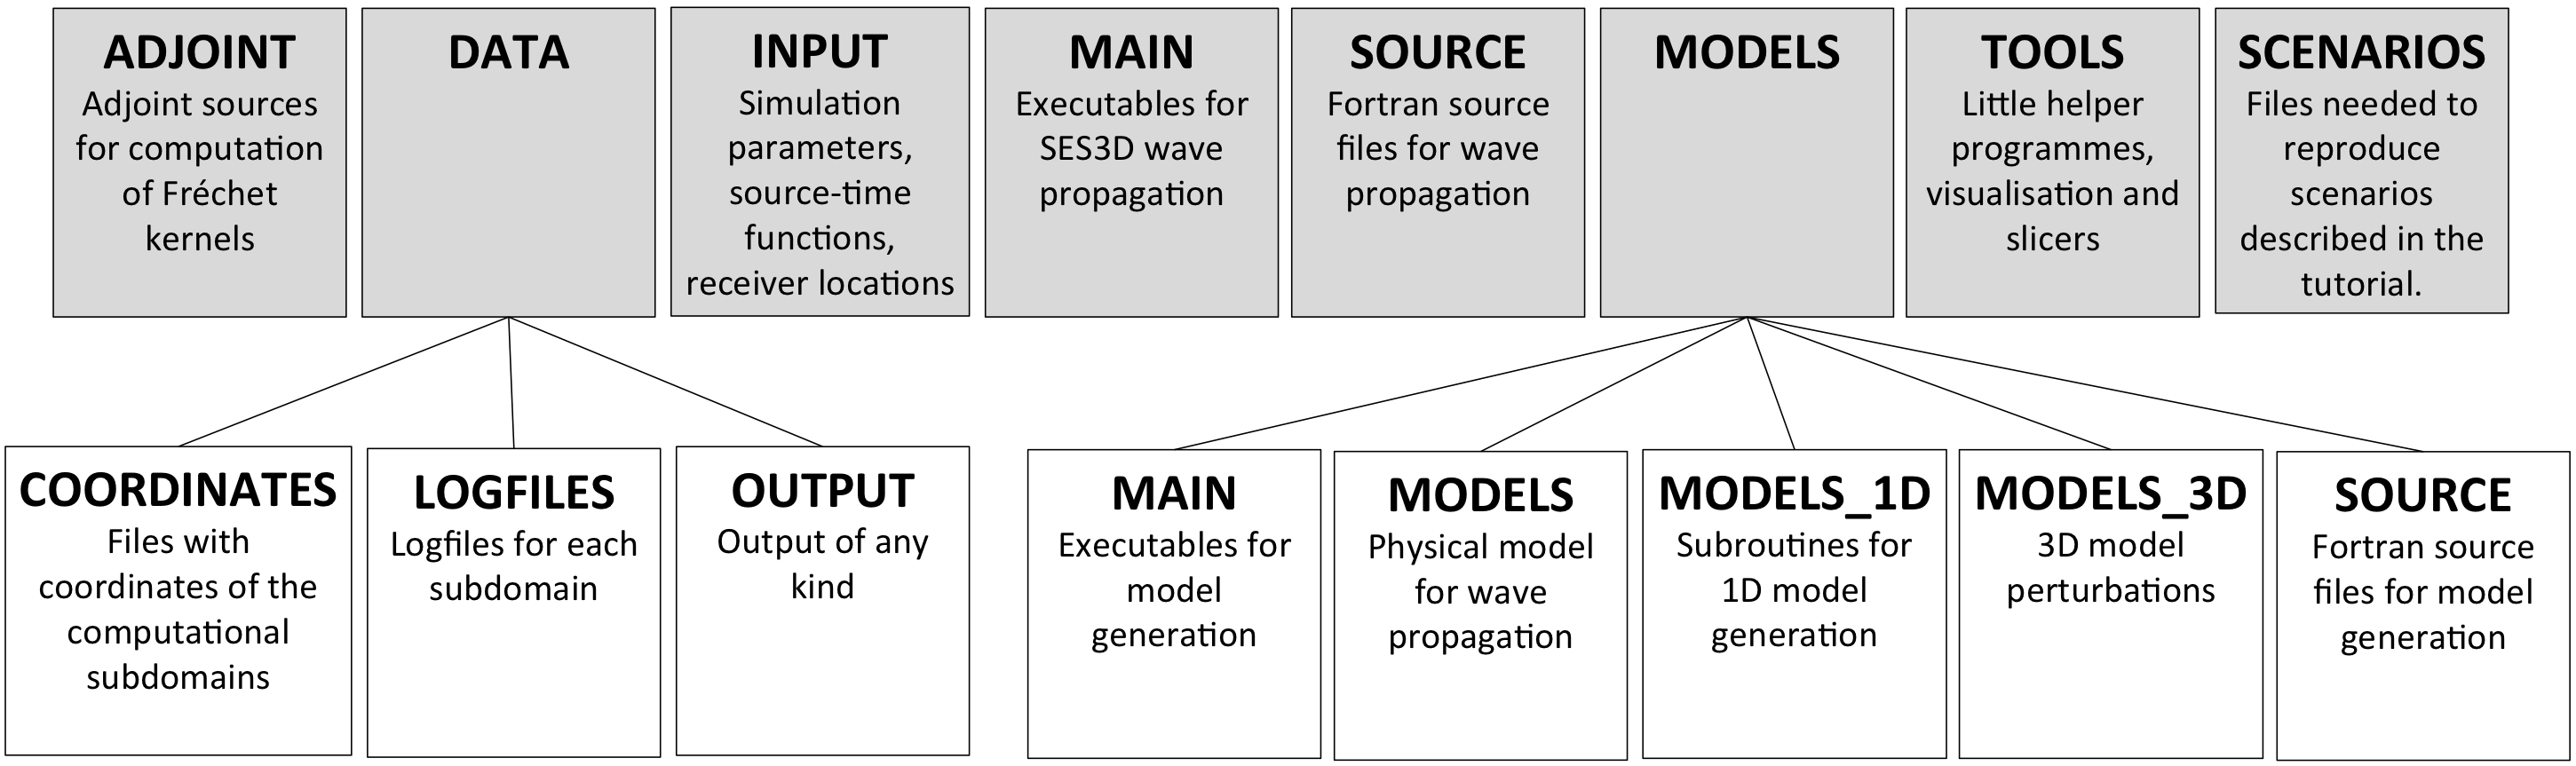
\includegraphics{Figures/directory_structure.png}}
\caption{\SES directory structure. See the text for detailed descriptions.}\label{F:directory_structure}
\end{figure}
\end{center}
%========================================================================

%====================================================================
% Source files.
%====================================================================

\section{Source files for wave propagation}

The principal source files for the wave propagation simulation and the computation of Fr\'{e}chet kernels can be found in the directory \texttt{SOURCE}. These are:\\[5pt]
\texttt{ses3d\_main.f90:} Initialisation of MPI, open logfiles, call subroutines for initialisation, call subroutines to iteratively advance the wavefield, monitor PML stability, write intermediate wave field in adjoint runs, clean up MPI and close files at the end of the iteration.\\[5pt]
\texttt{ses3d\_modules.f90:} Definition of variables and parameters.\\[5pt]
\texttt{ses3d\_input.f90:} Read parameter files \texttt{Par\_*}, read \texttt{boxfile} (contains information concerning the parallelisation), read 3D model parameters, read source time functions (\texttt{stf\_*}), read receiver locations (\texttt{recfile\_*}), read adjoint source locations (\texttt{ad\_srcfile}).\\[5pt]
\texttt{ses3d\_init.f90:} Set up grid point geometry, make mass matrix, compute receiver locations in unit cube coordinates, compute point source location in unit cube coordinates, read adjoint source
time functions, initialise PML damping profiles.\\[5pt]
\texttt{ses3d\_evolution.f90:} Propagate dynamic fields one time step forward.\\[5pt]
\texttt{ses3d\_grad.f90:} Compute Fr\'{e}chet kernels.\\[5pt]
\texttt{ses3d\_output.f90:} Collection of subroutines to write seismograms, store intermediate wave fields, write wave field snapshots and write Fr\'{e}chet kernels.\\[5pt]
\texttt{ses3d\_miscellaneous.f90:} Subroutines to add external forces (single force, moment tensor source, adjoint sources) and for the communication between compute cores.\\[5pt]
The above source files must be compiled together, e.g. by running the script \texttt{s\_make} located in the \texttt{SOURCE} directory. \textbf{A recompilation is necessary after a change of
the parallelisation scheme, i.e. a change of the division of the spherical section into subsections.}\\[5pt]
The script \texttt{s\_make} compiles all source files and combines them into the executables \texttt{ses3d.exe} located in the directory \texttt{MAIN}. Executing \texttt{ses3d.exe}
starts the forward or adjoint wave propagation.

%====================================================================
% Variable style.
%====================================================================

\section{Variable style and nomenclature of 3D fields}\label{S:variables}

In \SES, dynamics fields (velocity, stress, strain, material parameters, etc.) are implemented in the form of six-dimensional arrays. This is illustrated in figure \ref{F:variables} with the example of the
$\theta$-component velocity field. The first three dimensions of the array correspond to the element indices within a spherical subsection in $\theta$-, $\phi$- and radial directions. Note that
the radial index increases from the surface, where it is equal to $0$, towards greater depth. The last three indices are used to address the nodes within one element.\\[5pt]
Throughout \SES, $\theta$-components (colatitude) are labelled with \texttt{x}, $\phi$-components (longitude) with \texttt{y} and radial components with \texttt{z}. This is intended to keep the variable names short.
%========================================================================
\begin{center}
\begin{figure}
\center\scalebox{0.25}{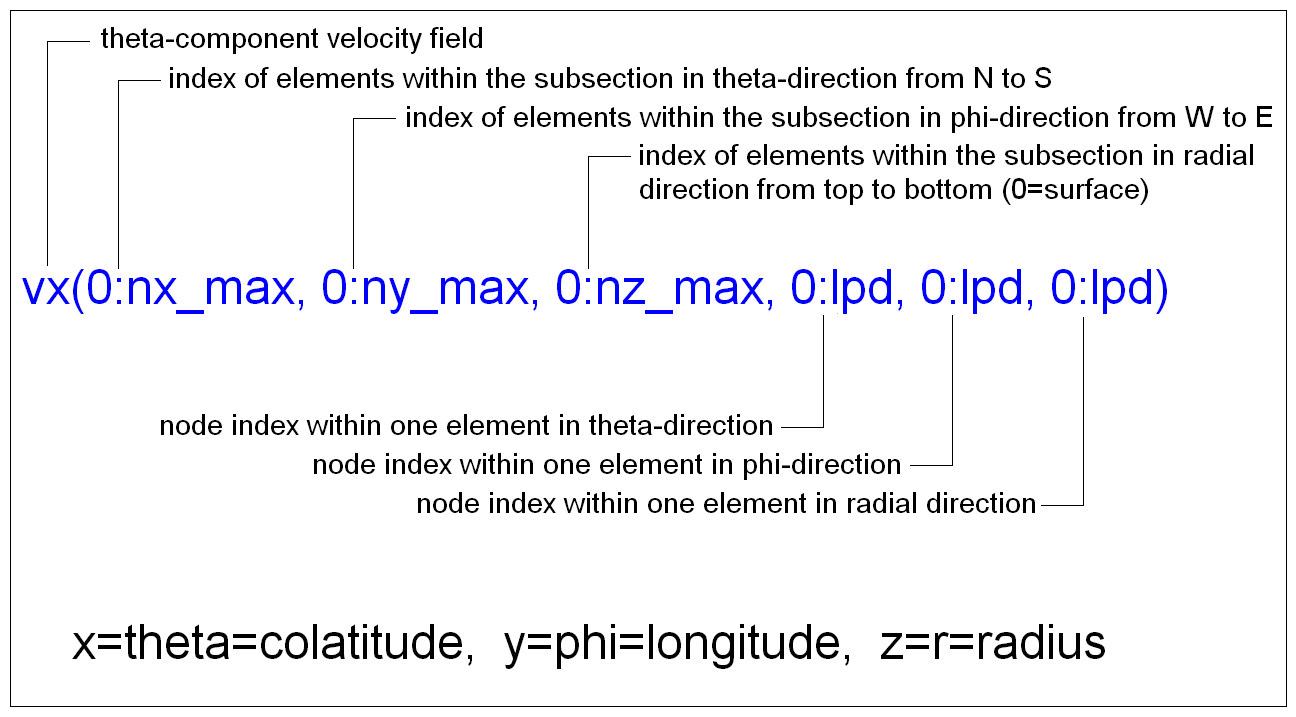
\includegraphics{Figures/variables.png}}
\caption{Structure and nomenclature of the dynamic fields in \SES. The example is for the velocity field in colatitudinal ($\theta$) direction.}\label{F:variables}
\end{figure}
\end{center}
%========================================================================

%====================================================================
% Calls to caution.
%====================================================================

\section{Calls to caution}\label{S:caution}

Each numerical method needs to be handled with care, and \SES is no exception. The following paragraphs are concerned with some of the difficulties that a user may encounter when working with \SES. It is generally recommended to assess the accuracy of numerical solutions by comparing them to semi-analytical solutions that exist for simplified models, e.g. radially symmetric Earth models.

\subsection{Absorbing boundaries}

\SES avoids unphysical reflections from the lateral and lower boundaries of the spherical section using a variant of the perfectly matched layers technique, called the method of anisotropic perfectly matched layers (APML, e.g. Teixeira \& Chew, 1997). It consists in the modification of the elastic wave equation within a narrow region along the unrealistic boundaries of the spherical section. The mathematical details of this method are explained in section \ref{S:absbound_theo}.\\[5pt]
The width of the absorbing boundary region, in terms of the number of elements, is specified by the parameter \texttt{pml} in the \texttt{ses3d\_modules.f90} source file. A good choice is \texttt{pml=3}, i.e. an absorbing boundary layer that is three elements wide.\\[5pt]
Within the absorbing layer, incoming waves are attenuated. This means that one should place neither receivers nor sources within the boundary layer. It is recommended to have at least two elements between the absorbing layer and receivers and sources.\\[5pt]
Contrary to what their name suggests, perfectly matched layers are not perfect. The imperfection comes in the form of two undesirable phenomena: (1) Incident waves are not completely absorbed by the absorbing layers. This means that small unphysical reflections will always be present. These can be minimised by placing sources and receivers further away from the boundaries. (2) All variants of the perfectly matched layers technique are long-term unstable. This means that the wavefield amplitudes may grow indefinitely for very long simulations, where the term \emph{very long} is not very well defined. 

\subsection{Seismic discontinuities and the crust}\label{S:crust}

Realistic Earth models typically contain discontinuities. Spectral-element solutions are correct only when discontinuities coincide with the edges of elements, such that the shared boundary
nodes take the different values from each side of the discontinuity. The inflexible grid of \SES is not always capable of accounting for discontinuities in the exact way. This means that discontinuities of the material properties may be located in the interior of elements. As a result, the numerical solutions may not be as exact as they would be in the case of perfectly honoured discontinuities. This effect is difficult to quantify, and it mostly concerns surface waves.\\[5pt]
A related problem is the implementation of thin crustal layers that may be thinner than a layer of elements. This can also produce inaccurate numerical solutions.\\[5pt]
Difficulties with thin crustal layers and discontinuities can most easily be avoided by the implementation of long wavelength equivalent models (e.g. Capdeville \& Marigo, 2007, 2008; \href{http://www.geo.uu.nl/~fichtner/papers/2008_fichtner_DCM.pdf}{Fichtner \& Igel, 2008}).

\subsection{The poles and the core}

Since \SES operates in the natural spherical coordinate system, one must exclude the poles and the core from the computational domain. A the centre of the Earth, spatial derivatives in spherical coordinates are singular. Also, the elements become very small near the poles and near the core, so that the time step \texttt{dt} must be chosen very small. To run \SES efficiently, the spherical sections should not be deeper than $\sim 3000$ km and not closer than $\sim 20^\circ$ to one of the poles.